\documentclass[twocolumn]{aastex62}
\emergencystretch=1.em

\usepackage{amsmath,amsthm,amsfonts,amssymb,bm}
% for big dot
\makeatletter
\newcommand*\bigcdot{\mathpalette\bigcdot@{.5}}
\newcommand*\bigcdot@[2]{\mathbin{\vcenter{\hbox{\scalebox{#2}{$\m@th#1\bullet$}}}}}

\usepackage{listings}
\usepackage{multirow}
\usepackage{color}

%\usepackage{subfigure}
\usepackage{textcomp}
\usepackage{epstopdf}
\usepackage{natbib}
\usepackage{commath}
\hypersetup{breaklinks}
\DeclareMathOperator{\arccosh}{arccosh}
\newcommand \figPath{./}
\newcommand \redColor{\color{red}}
\renewcommand\labelenumi{(\roman{enumi})}
\renewcommand\theenumi\labelenumi

\usepackage{algorithm,algcompatible}
\DeclareMathOperator*{\argmax}{\arg\!\max}
\algnewcommand\INPUT{\item[\textbf{Input:}]}
\algnewcommand\OUTPUT{\item[\textbf{Output:}]}

\makeatother
%\newcommand{\jcap}{JCAP}

\begin{document}
\title{Sparsity Weak Lensing $3$- Mass Reconstruction}
%\author{Xiangchong Li}
%\affiliation{Department of Physics, University of Tokyo, Tokyo 113-0033, Japan}
%\affiliation{Kavli Institute for the Physics and Mathematics of the Universe (WPI),\\
%University of Tokyo, Kashiwa 277-8583, Japan}
%\author{Masamune Oguri}
%\affiliation{Department of Physics, University of Tokyo, Tokyo 113-0033, Japan}
%\affiliation{Kavli Institute for the Physics and Mathematics of the Universe (WPI),\\
%University of Tokyo, Kashiwa 277-8583, Japan}
%\affiliation{Research Center for the Early Universe, University of Tokyo, Tokyo 113-0033, Japan}
%\author{Wentao Luo}
%\affiliation{Kavli Institute for the Physics and Mathematics of the Universe (WPI),\\
%University of Tokyo, Kashiwa 277-8583, Japan}
%\author{HSC Collaboration}
%\noaffiliation
%\email{xiangchong.li@ipmu.jp}

\begin{abstract}

\end{abstract}

\section{Introduction}
Light from distant galaxies is distorted by the intervening inhomogeneous density distribution along the line-of-sight
due to the influence of gravity and the shapes of the background galaxies are coherently sheared due to the lensing effect.
Such effect, which is known as weak lensing, imprints the information of foreground mass density distribution to the
background galaxy images and offers a direct probe into the mass density distribution in the universe \citep[see][for recent 
reviews]{revKilbinger15,revRachel17}.

Mathematically, the shear field ($\gamma$) measured distant galaxies is a linear mapping of the density contrast ($\delta$)
\begin{equation}
 \gamma=\mathbf{T} \delta,
\end{equation}
where $\mathbf{T}$ is the transformation operator. The transformation operator ($\mathbf{T}$) includes not only physical lensing
effect but it also includes observational systematic effects.

In order to fully reconstruct the $3$-D mass density distribution ($\delta$) from the $3$-D shear field ($\gamma$) 
observed from distorted galaxy images, a premise is take that the density field can be decomposed into a set of models
\begin{equation}
 \delta= \mathbf{\Phi} x,
\end{equation}
where $\mathbf{\Phi}$ is the transformation operator from the model space to the mass density and $x$ is the projector. 
In the previous works, Starlets (wavelets transform) and sinusoidial functions (Fourier transform) have been used to 
modeled the density field . 

Subsequently, an ill-posed inverse problem
\begin{equation}
\rm{min}_x\{\norm{\gamma - \mathbf{T\Phi} x}_2^2+ C(x)\},
\end{equation}
need to be solved to reconstruct the mass density map, where $C(x)$ is the regulation term which makes the ill-posed 
inversion solvable. The $l^1$ sparsity regulation and the $l^2$ ridge regulation have been applied to the mass density 
map reversion problem. In their application, the $l^1$ sparsity regulation ($\norm{x}^1_1$) is combined with Starlets modeling 
\citep{LSS-massMap-Glimpse3D-Leonard2014} and the $l^2$ ridge regulation ($\norm{x}^2_2$) is combined with sinusoidial modeling\footnote{It 
is also known as Wiener filter.} \citep{LSS-massMap-Wiener-Simon2009}. See \citet{HSC1-massMaps} for a recent application 
of \citet{LSS-massMap-Wiener-Simon2009} in the Hyper Suprime-Cam Survey \citep{HSC1-data}.

We propose to use NFW halos \citep{halo-NFW1997ApJ} to model the density contrast field and construct the density contrast 
field with $l^1$ sparsity regulation.


This paper is organized as follows.
Section \ref{sec:Method} proposes the new method for $3$-D mass map reconstruction.
Section \ref{sec:Sim} introduces the realistic simulations we use to test the new method.
Section \ref{sec:Res} presents the results of our method on the simulations.
Section \ref{sec:Sum} summarizes and discusses the future development of the method.

\section{Methodology}
\label{sec:Method}

In this section, we first review how the foreground density contrast induces the weak lensing shear distortion on background 
galaxies in section \ref{subsec:method-delta2shear}.
After that, we describe several systematic effects which exist in real observation mathematically. The systematic effects 
include photo-$z$ uncertainty (section \ref{subsec:method-photoz}), smoothing (section \ref{subsec:method-smoothing}),
mask and noise (section \ref{subsec:method-msknoise}) and pixelation (section \ref{subsec:method-pix}).

Subsequently, we propose a novel method to reconstruct the $3$-D density contrast field from the weak lensing shear 
distortion field. 
With the premise that the density field can be decomposed into NFW halos and point masses, we build up a dictionary using 
NFW models and point mass models in section \ref{subsec:method-dictionary}.
The models in our dictionary are used to fit the shear field and the optimal fit is determined by minimizing a loss function. 
As shown in section \ref{subsec:method-lossfun} the loss function is composed of a normal chi-$2$ term, a $l_1$ sparsity 
constrain and a quadratic total square variance constrain.
The minimum of the loss function is achieved with the pathwise coordinate descent algorithm in section \ref{subsec:method-pathwise}.

\subsection{Density Contrast to Shear}
\label{subsec:method-delta2shear}

\begin{figure*}
    \includegraphics[width=0.95\textwidth]{nfwlet-atom-2D.pdf}
    \caption{The NFW models with different scale radius ($r_s$). The first row shows the NFW models in Fourier
            space and the second row shows the NFW model in Real space.}
\end{figure*}

The lensing convergence $\kappa$ at the comoving distance $\chi_s$ caused by the foreground inhomogeneous
density distribution at the comoving distance $\chi_l$ ($\chi_l< \chi_s$) along the line-of-sight is
\begin{equation}
\kappa(\vec{\theta},\chi_s)=\frac{3H_0^2\Omega_M}{2 c^2} \int_0^{\chi_s} d\chi_l \frac{\chi_l \chi_{sl}}{\chi_s}
\frac{\delta(\vec{\theta},\chi_l)}{a(\chi_l)},
\end{equation}
\citep{LSS-massMap-Glimpse3D-Leonard2014}.
where $\chi$ refers to the comoving distance, $\delta=\rho(\vec{\theta},\chi_l)/\bar{\rho}-1$ is the density contrast
at the position of lens, $H_0$ is the Hubble parameter, $\Omega_M$ is the matter density parameter, $c$ is the speed
of light, and $a(\chi_l)$ is the scale parameter at the lens position.

Substitute comoving distance ($\chi$) with redshift ($z$)
$z$ and we have
\begin{equation}\label{eq-delta2kappa}
\kappa(\vec{\theta},z_s)=\int_0^{z_s} dz_l \delta_{c}^{-1}(z_l,z_s)\delta(\vec{\theta},z_l).
\end{equation}
$K(z_l,z_s)$ as the lensing kernel defined as
\begin{equation}
K(z_l,z_s) =
\begin{cases}
\frac{3H_0\Omega_M}{2 c} \frac{\chi_l \chi_{sl} (1+z_l)}{\chi_{s} E\left(z_l\right)} & (z_s>z_l),\\
0&(z_s \leq z_l).
\end{cases}
\end{equation}

As shown in \citet{massMap-KS1993}, the shear distortion is related to the kappa field at the redshift plane as
\begin{equation}\label{eq-kappa2gamma}
\gamma^t(\vec{\theta},z_s) = \int  d^2 \theta' D(\vec{\theta}-\vec{\theta'}) \kappa(\vec{\theta'},z_s),
\end{equation}
where
\begin{equation}
D(\vec{\theta})=-\frac{1}{\pi}(\theta_1-i\theta_2)^{-2}.
\end{equation}
Here we denote the true shear distortion as $\gamma^t$ to distinguish the observed shear signal with systematics which 
will be introduced in the following subsections.

Combining equation (\ref{eq-delta2kappa}) with equation (\ref{eq-kappa2gamma}), the true shear signal is derived as
\begin{equation}\label{eq-delta2gamma-z}
\gamma^t(\vec{\theta},z_s) = \int_0^{z_s} \frac{dz_l}{\delta_{c}(z_l,z_s)} \int d^2 \theta' \vec{D}(\vec{\theta}-\vec{\theta'}) \delta(\vec{\theta'},z_l).
\end{equation}
Here we define the lensing functional as 
\begin{equation}
\mathbf{Q}=\int_0^{z_s} \frac{dz_l}{\delta_{c}(z_l,z_s)} \int d^2 \theta'  \vec{D}(\vec{\theta}-\vec{\theta'}),
\end{equation}
then eq. (\ref{eq-delta2gamma-z}) is simplified to $\gamma^t=\mathbf{Q}\delta$.

\subsection{Photo-$z$ Uncertainty}
\label{subsec:method-photoz}
\begin{figure}
 \includegraphics[width=0.5\textwidth]{nfwlet-atom-1D.pdf}
 \caption{The $1$-D slices of NFW models with different scale radius ($r_s=0,1,2,4,8$).}
\end{figure}

Since the photometric redshifts of source galaxies in the current large scale survey are estimated with 
a limited number of photometric bands, the estimated redshift of a single galaxy suffers from large uncertainty.
We denote the probability of a galaxies, with photo-$z$ estimated as $z_s$, being actually located at redshift
$z$ as $P(z|z_s)$.  Note that, in order to simplify the future calculation, we assume the variation of the PDF 
across the transverse plane is small and neglect such variation.

Taking the uncertainty of redshift into account, the shear signal changes to
\begin{equation}\label{eq-delta2gamma-poz}
\gamma^p(\vec{\theta},z) = \int dz_s P(z|z_s) \gamma^t(\vec{\theta},z_s).
\end{equation}
With the definition of photo-$z$ functional
\begin{equation}
\mathbf{P} = \int dz_s P(z|z_s),
\end{equation}
the relation between shear signal and density contrast is $\gamma^p=\mathbf{P} \mathbf{Q} \delta$.

\subsection{Smoothing}
\label{subsec:method-smoothing}

Since the observed galaxies have random irregular (unequally-spaced) distribution, it is necessary to smooth 
the shear signal in the observation. The smoothing is expressed as follows
\begin{equation}
\hat{\gamma}  = \frac{\sum_i  W(\vec{\theta}-\vec{{\theta}}_i,z-z_i) e_i}{\sum_i R_i W(\vec{\theta}-\vec{{\theta}}_i,z-z_i) },
\end{equation}
where $W(\vec{\theta},z)$ is a $3$-D smoothing kernel. $e_i$, $R_i$, $z_i$ and $\theta_i$ are the ellipticity, 
response, reshift, and transverse position of the `$i$-th' galaxy in the galaxy catalog.

$W(\vec{\theta},z)$ can be decomposed into a transverse component $W_T(\vec{\theta})$ and a line-of-sight component 
$W_\times(z)$
\begin{equation}
W(\vec{\theta},z)=W_T(\vec{\theta}) W_\times (z).
\end{equation}
In this paper, we set
\begin{equation}
\begin{split}
W_T(\vec{\theta}) &=\frac{1}{2\pi\beta^2}\exp(-\frac{|\vec{\theta}|}{2\beta^2}),\\
W_\times (z) &=
\begin{cases}
1/\Delta z& (|z|<\Delta z/2),\\
0& else.
\end{cases}
\end{split}
\end{equation}

With the approximation that the density of response $R$ and the density of galaxy number vary slowly on the smoothing scale
and the fact that $\int d^3r W(\vec{r})=1$, the smoothed shear is
\begin{equation}\label{eq-smooth-gamma}
\gamma^s(\vec{r})= \int d^3 r' W(\vec{r}-\vec{r'}) \gamma^p(\vec{r'})
\end{equation}

We define the smoothing functional as
\begin{equation}
\mathbf{W} = \int d^3 r' W(\vec{r}-\vec{r'}),
\end{equation}
and the relation between shear signal and density contrast is $\gamma^s=\mathbf{W} \mathbf{P} \mathbf{Q} \delta$.

\subsection{Mask and Noise}
\label{subsec:method-msknoise}

In real observations, the influence of mask and noise should also be taken into account. The final observed shear is
\begin{equation}\label{eq-delta2gamma-final}
\gamma(\vec{\theta},z)=M(\vec{\theta},z) \gamma^s(\vec{\theta},z) + \epsilon(\vec{\theta},z),
\end{equation}
where $\epsilon$ represents noise typically caused by random shape of intrinsic galaxies and such noise is modeled 
as uncorrelated Gaussian noise. $M(\vec{\theta},z_s)$ is the mask function.

With the definition of masking functional,
\begin{equation}
\mathbf{M}= \int d^3 r' M(\vec{r'}) \delta_D(\vec{r}-\vec{r'}),
\end{equation}
where $\delta_D(\vec{r})$ is $3$-D Dirac delta function, we can write equation (\ref{eq-delta2gamma-final}) into
\begin{equation}\label{eq-delta2gamma-operator-final}
\gamma =\mathbf{M} \mathbf{W} \mathbf{P} \mathbf{Q} \delta + \epsilon.
\end{equation}

\subsection{Dictionary}
\label{subsec:method-dictionary}
\begin{figure}
 \centering
 \includegraphics[width=0.5\textwidth]{photo-z_binning.pdf}
 \caption{The source galaxies are binned into $10$ redshift bins according to their mlz best photo-$z$ estimation. 
        The blue histogram is the number distribution of the best photo-$z$ estimation. The vertical dashed lines 
        are the bounds of bins. The galaxies are evenly distributed in each bins.}
\end{figure}

$N$-body simulations show that the dark matter to be largely distributed in halos connected by filaments, therefore,
we assume that the density contrast field can be decomposed into multi-scaled NFW halo \citep{halo-NFW1997ApJ} and
point mass at different positions
\begin{equation}
\delta(\vec{r}) = \sum_{s=0}^{N} \int d^3 r' \phi_s(\vec{r}-\vec{r'}) x_s(\vec{r'})\\
\end{equation}
where $\phi_0$ is $3$-D Dirac delta function to model point masses
\begin{equation}
\phi_0(\vec{r})= \delta_D(\theta_1) \delta_D(\theta_2) \delta_D(z).
\end{equation}
Since the scale of halo is much less than the reachable redshift resolution, we neglect the depth of halo on the 
line-of-sight direction following \citep{LSS-massMap-Glimpse3D-Leonard2014}. On the other hand, in the transverse directions, 
the surface density profiles of NFW halos with scale $\theta_\alpha$ and truncation radius $c \theta_\alpha$ 
\citep{haloModel-TJ2003-3pt} are used to model halos, where $c$ is generally known as concentration of NFW halo.  

\begin{equation}
\begin{split}
\phi_\alpha(\vec{r}) =&\frac{f }{2 \pi \theta_\alpha^2 } F(|\vec{\theta}|/\theta_\alpha) \delta_D(z),\\
&  (s=1..N)
\end{split}
\end{equation}
where
\begin{equation}
F(x)=
\begin{cases}
-\frac{\sqrt{c^2-x^2}}{(1-x^2)(1+c)} + \frac{\arccosh \left(\frac{x^2+c}{x(1+c)}\right)}{(1-x^2)^{3/2}}  & (x<1),\\
\frac{\sqrt{c^2-1}}{3(1+c)} (1+\frac{1}{c+1}) & (x=1),\\
-\frac{\sqrt{c^2-x^2}}{(1-x^2)(1+c)} + \frac{\arccos\left(\frac{x^2+c}{x(1+c)}\right)}{(x^2-1)^{3/2}} & (1<x\leq c),\\
0& (x>c).
\end{cases}
\end{equation}
$f=1/[\ln (1+c)-c/(1+c)]$, and $x_\alpha$ is the corresponding projection coefficient of the density contrast
field onto our basis NFW model.

We define the projection parameters set as $x=\begin{pmatrix}
x_{[0]}\\
x_{[1]}\\
...\\
x_{[N]}
\end{pmatrix}$, and the dictionary transforming functional as
\begin{equation}
\mathbf{\Phi}=\begin{pmatrix}
\int d^3r\phi_0(\vec{r}) ~\int d^3r \phi_1(\vec{r})~ ...~\int d^3r \phi_{N}(\vec{r})
\end{pmatrix}.
\end{equation}
Then we write equation (\ref{eq-delta2gamma-operator-final}) into
\begin{equation}\label{eq-alpha2gamma-operator}
\gamma=\mathbf{M}\mathbf{P}\mathbf{Q}\mathbf{\Phi} x +\epsilon,
\end{equation}
where $\epsilon(\vec{r})$ is the error from the shear measurement which includes contributions from both random
galaxy orientations and photon noise.

For simplicity, we denote $\mathbf{A}=\mathbf{M}\mathbf{P}\mathbf{Q}\mathbf{\Phi} $ and eq. (\ref{eq-alpha2gamma-operator})
reduces to 
\begin{equation}\label{eq-x2gamma-simple}
\gamma=\mathbf{A} x +\epsilon.
\end{equation}

\subsection{Pixelization}
\label{subsec:method-pix}
We pixelize the smoothed shear field ($\gamma$) into a $N_\theta \times N_\theta \times N_s$ grid, where $N_\theta$ 
is the number of pixels of two orthogonal axes of the transverse plane and $N_s$ is the number of pixels of the 
line-of-sight axis. $\gamma_{\alpha}$ is used to denote the value recorded on pixel with index $\alpha$, where $\alpha=
1..N_\theta \times N_\theta \times N_s$. The grid on the transverse plan is equally spaced so that we can perform the Fast 
Fourier Transform (FFT) on the transverse plan.

Similarly, we pixelize each frame \footnote{Here we have $N$ dictionary frames in total} of the projector into a $N_\theta 
\times N_\theta \times N_l$ grid. The pixelization on the transverse plan of each parameter frame is exactly the same as 
that of the observational frame. $N_l$ is the number of pixels on the line-of-sight axis. $x_{\beta}$ is used to denote the 
value recorded on pixel with index $\beta$, where $\beta=1..N_\theta \times N_\theta \times N_l \times N$.

With Einstein notation, eq. (\ref{eq-x2gamma-simple}) reduces to
\begin{equation}
\gamma_{\alpha} = A_{\alpha\beta} x_{\beta} + \epsilon_{\alpha},
\end{equation}
where $\epsilon_{\alpha}$ refers the noise ($\epsilon$) on the pixel of index $\alpha$.

\subsection{Loss Function with Constrains}
\label{subsec:method-lossfun}
\begin{figure}
 \centering
 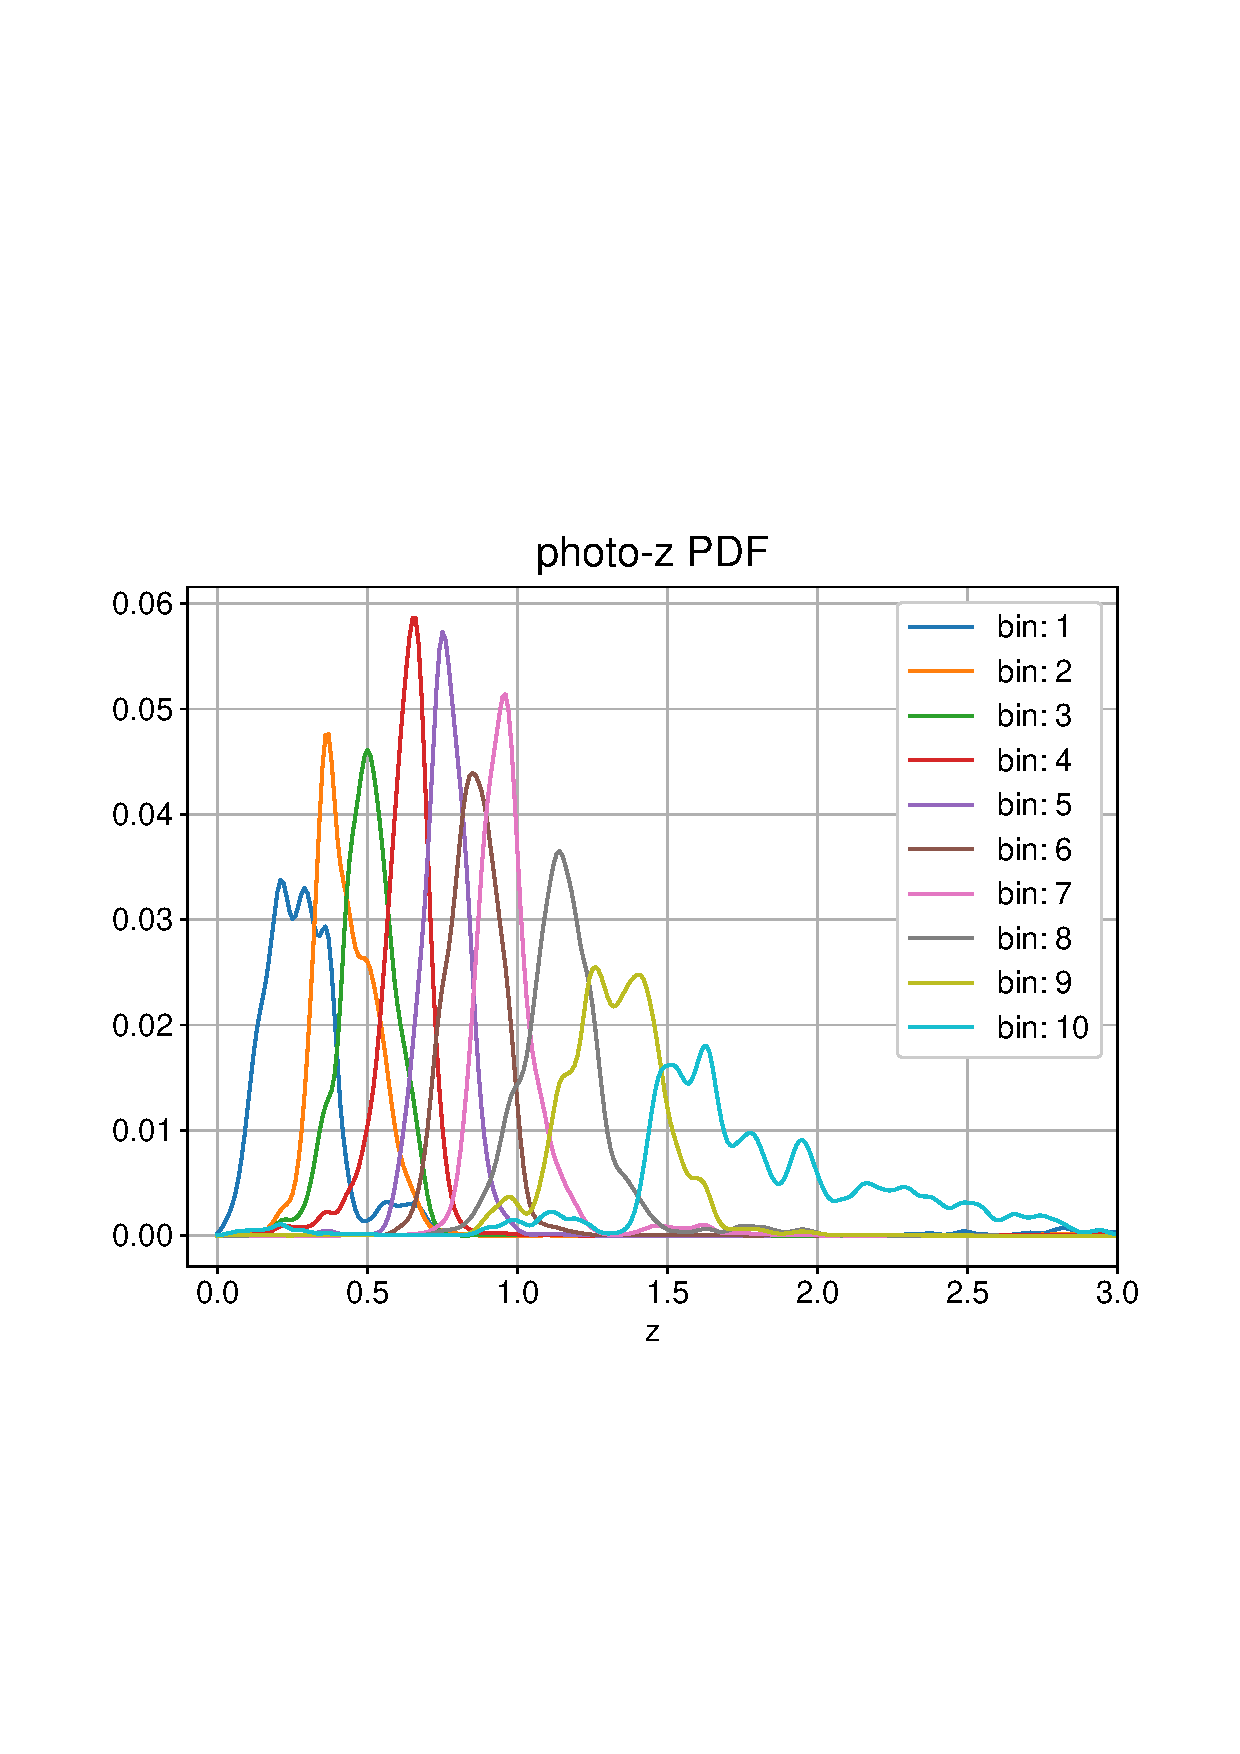
\includegraphics[width=0.5\textwidth]{mlz-poz.pdf}
 \caption{The PDF of photo-$z$ error for $10$ source redshift bins.}
\end{figure}

We define the loss function as
\begin{equation}\label{eq-lossFun}
L(x) = \frac{1}{2} \norm{\gamma-\mathbf{A}x}^2_2 + \frac{1}{2}\tau \mathrm{TSV}(x)+\lambda \sigma \norm{x}_1 ,
\end{equation}
where $\norm{\bigcdot}_1$ and $\norm{\bigcdot}_2$ refer to the $l^1$ norm and $l^2$ norm, respectively. 
$\mathrm{TSV}(x)$ refers to the total square variance of the first dictionary frame, which is defined as
\begin{equation}
\begin{split}
\mathrm{TSV}(x) =\int d^2 \theta dz (\frac{\partial x}{\partial \theta_1})^2+\int d^2 \theta dz (\frac{\partial x}{\partial \theta_2})^2.
\end{split}
\end{equation}
The total square variance can be expressed in a quadratic form as
\begin{equation}
\mathrm{TSV}(x)=\norm{\frac{\partial x}{\partial \theta_1}}^2_2+\norm{\frac{\partial x}{\partial \theta_2}}^2_2.
\end{equation}

The $l^1$ term is the sparsity constrain. The TSV term constrains on the smoothness of the mass distribution in the 
point mass dictionary frame.

The loss function defined on the pixelized data is
\begin{equation}
\begin{split}
L(x)&=\frac{1}{2}(\gamma_{\alpha}-A^{*}_{\alpha\beta}x_{\beta})(\gamma_{\alpha}-A_{\alpha\mu}x_{\mu})\\
&+\frac{\tau}{2}[(D^{1}_{\alpha\beta} x_{\beta})(D^{1}_{\alpha\mu}x_{\mu})
+ (D^{2}_{\alpha\beta} x_{\beta})(D^{2}_{\alpha\mu}x_{\mu})] \\
&+ \lambda\sigma_\beta \norm{x_\beta}_1,
\end{split}
\end{equation}
where $\mathbf{D^1}$ and $\mathbf{D^2}$ and difference operator on $\theta_1$ and $\theta_2$ directions, respectively.


\subsection{Pathwise Coordinate Descent Algorithm}
\label{subsec:method-pathwise}
\begin{figure}
 \centering
 \includegraphics[width=0.5\textwidth]{lensing_efficiency.pdf}
 \caption{The blue line shows the normalized lensing efficiency for lens bin at $z_{l}=0.51$.
 The orange line is the normalized lensing efficiency while taking into account the photo-$z$ uncertainty.
 The green data points show the averaged $\kappa$ field for different redshift bins in the simulation.}
\end{figure}

The loss function can be separated into a summation of a quadratic term and a $l^1$ term as
\begin{equation}
 L(x)=G(x)+\lambda\sigma_{\beta}\norm{x_{\beta}}_1.
\end{equation}
The quadratic term is defined as
\begin{equation}
\begin{split}
 G(x)&=\frac{1}{2}(\gamma_{\alpha}-A^{*}_{\alpha\beta}x_{\beta})(\gamma_{\alpha}-A_{\alpha\mu}x_{\mu})\\
&+\frac{\tau}{2}[(D^{1}_{\alpha\beta} x_{\beta})(D^{1}_{\alpha\mu}x_{\mu})
+ (D^{2}_{\alpha\beta} x_{\beta})(D^{2}_{\alpha\mu}x_{\mu})],
\end{split}
\end{equation}

Many algorithms have been proposed to find the minima of this kind of loss function. We base our method on the 
coordinate descent algorithm \citep{coordinateDescent-Wright2015} which is described as follows.
Firstly, we initialize the projector as $x^{(1)}=0$. According to the coordinate descent algorithm, we subsequently 
update the projector ($x$) along the direction of one specific coordinate ($i$) as
\begin{equation}
x^{(n+1)}_{i}=\mathrm{ST}_{\lambda\sigma_{i}} (x^{(n)}_{i} -\frac{\partial_i G(x^{(n)})}{A_{\alpha i}A_{\alpha i}+4\tau}), 
\end{equation}
where $\mathrm{ST}$ is the soft thresholding function defined as
\begin{equation}
\mathrm{ST}_{\lambda} (x) = \mathrm{sign} (x) \max (\abs{x}-\lambda,0),
\end{equation}
and the projector along the other coordinates are kept the same. The minima is finally approached by iteratively updating 
along each coordinate for multiple times. 

To simplify the notation, here we define the projector difference for the $n$-th iteration as
\begin{equation}
 \Delta x ^{(n)} = -\frac{\bigtriangledown G(x^{(n)})}{A_{\alpha i}A_{\alpha i}+4\tau},
\end{equation}
where $\bigtriangledown G(x^{(n)})$ refers to the gradient of quadratic function $G$ at $x^{(n)}$. The signal to noise ratio 
(SNR) of the projector difference is defined as $s^{(n)}=\Delta x ^{(n)}/\sigma$.


In our algorithm, the coordinate descent algorithm in conducted in a pathwise manner \citep{pathwise-Friedman2007}. 
We begin with a regulation parameter 
($\lambda^{(1)}$) which is slightly smaller than the maximum coordinate of $s^{(1)}$ (denoted as $s_{\rm{max}}^{(1)}$) so that 
in the first iteration, we only update on the coordinate with the maximum SNR. Then, we find the maximum projector difference 
SNR of the second iteration ($s_{\rm{max}}^{(2)}$) and update the regulation parameter to $\lambda^{(2)}$, where $\lambda^{(2)}$
is slightly smaller than $s_{\rm{max}}^{(2)}$.

The algorithm is fully described in Algorithm \ref{alg-1}.

\begin{algorithm}[H]
    \label{alg-1}
    \caption{Our Algorithm}
  \begin{algorithmic}[1]
    \INPUT   $\gamma$: Complex $3$-D array of shear
    \OUTPUT  $\delta$: $3$-D array of density contrast
    \STATE \textbf{Initialization} ‎$x^{(1)} = 0$, $\lambda^{(1)} = 100$
    \WHILE{$i \leq N_{\rm{iter}}$}
      \STATE 
      \STATE 
      \STATE 
      \STATE 
    \ENDWHILE
  \end{algorithmic}
\end{algorithm}


\section{Simulation}
\label{sec:Sim}
This section simulates lensing shear fields induced by a group of dark matter halos with various halo mass and redshifts.
HSC-like shape measurement error and photo-$z$ error are added to the shear field.

\subsection{Weak Lensing Fields}

We simulate weak lensing shear fields of NFW halos according to \citet{haloModel-TJ2003-3pt}
and sample halos in the mass-redshift plane as shown in Figure \ref{fig:mass-redshift}.
We assume a dependency of the concentration on the mass and the redshift of a halo
\begin{equation}
c_{h}=6.02\times(\frac{M_{200}}{10^{13} M_{\odot}})^{-0.12}(\frac{1.47}{1.+z_h})^{0.16}.
\end{equation}


\begin{figure}[!ht]
 \centering
 \includegraphics[width=0.45\textwidth]{mass-redshift-sampling.pdf}
 \caption{The sampling points of halos in the mass-redshift plane.}
 \label{fig:mass-redshift}
\end{figure}

\subsection{HSC-like Errors}
\subsubsection{Shear Measurement Error}
\begin{figure}[!ht]
 \centering
 \includegraphics[width=0.45\textwidth]{shapeMeasurementError-HSCY1.pdf}
 \caption{HSC-like measurement error on the first component of shear ($g_1$).}
 \label{fig:mass-redshift}
\end{figure}

\subsubsection{Photo-$z$ Error}

\section{Results}
\label{sec:Res}

\begin{figure*}
\centering
\includegraphics[width=0.3\textwidth]{resultExp-tau010.png}
\includegraphics[width=0.3\textwidth]{resultExp-tau015.png}
\includegraphics[width=0.3\textwidth]{resultExp-tau020.png}
\caption{The density map reconstructed for a halo with mass=$3.16\times 10^14 M_{\sun}/h$, $z=0.51$. The left panel shows
the results with $\tau=0.10$, the middle panel is the result for $\tau=0.15$, the right panel is for $\tau=0.20$.}
\end{figure*}


\subsection{Detection Rate}

\subsection{Mass and Redshift Estimation}


\section{Summary}
\label{sec:Sum}

\begin{figure}[!ht]
 \centering
 \includegraphics[width=0.45\textwidth]{noise_std_map_pix.pdf}
 \caption{The standard deviation map of shear measurement error for the fifth source bin ($0.69 \leq z < 0.80 $).}
\end{figure}

\bibliographystyle{aasjournal}
\bibliography{weak_lensing,lensCat,cosmoSim,cmbObs,gglens,shearCor,massMap,other,optimize}

\appendix
\end{document}
